\chapter{Análise e Desenvolvimento de Modelos de Usuários Baseado em Múltiplos Domínios para Sistemas de Recomendação}
\label{cap:multiDomainUserModel}



Os processos de software são um conjunto de atividades que levam ao desenvolvimento de um sistema. Esses processos são complexos e não são desenvolvidos necessariamente de uma única forma \citep{Sommerville10}. O processo de software forma a base para o gerenciamento e controle de projetos de software e estabelecem o contexto no qual métodos técnicos são aplicados, produtos do trabalho (modelos, documentos, dados, relatórios, formulários, etc.) são produzidos, os marcos são estabelecidos, a qualidade é assegurada e modificações são adequadamente geridas \citep{Pressman:2009:SEP:1593949}.

Neste capítulo, nós apresentaremos os requisitos funcionais e não funcionais para uma sistema que coleta informações de múltiplos domínios (filmes e livros) sobre usuários a partir do Facebook\footnote{http://www.facebook.com} de forma automática. São discutidos aspectos de sua arquitetura e tecnologias utilizadas. Também é mostrada a ferramenta em operação, discutindo aspectos de seu funcionamento. Por fim, é apresentado um sumário do capítulo.



\section{Requisitos}

Os requisitos de software são as descrições do que o sistema deve fazer, os serviços que ele fornece e as restrições em sua operação \citep{Sommerville10}. O objetivo desta fase é coletar informações sobre o problema a ser resolvido, que refletem as necessidades do cliente para um sistema.

Os requisitos de software são frequentemente classificados como requisitos funcionais e requisitos não funcionais:

\begin{enumerate}
	\item{\textbf{Requisitos funcionais}: São recursos que o sistema deve fornecer, como o sistema deve reagir para entradas específicas, e como o sistema deve se comportar em determinadas situações.}
	
	\item{\textbf{Requisitos não funcionais}: São restrições dos serviços ou funções fornecidas pelo sistema. Inclui restrições de tempo, restrições no processo de desenvolvimento, e restrições impostas por padrões.}
\end{enumerate}

Esta seção especifica os requisitos do sistema desenvolvido como proposta deste trabalho, fornecendo informações necessárias para o projeto e implementação.

Para identificação dos requisitos foram adotadas as seguintes convenções: [RF0XX] para requisitos funcionais, e [RNF0XX] para requisitos não funcionais. Também foram atribuídas prioridades aos requisitos. As prioridades servem para indicar a relevância do requisito para o sistema proposto, e foram classificadas em: a) Essencial, são requisitos que precisam ser implementados impreterivelmente, indicando que sem este requisito o sistema não pode funcionar ou não atende o objetivo da proposta; b) Importante, são requisitos que o sistema pode funcionar, porém, de forma parcial; c) Desejável, são requisitos que não comprometem o funcionamento básico do sistema e que podem ser deixados para versões posteriores deste trabalho.

\subsection{Requisitos Funcionais}

A Tabela \ref{tab:req-funcionais} apresenta os requisitos funcionais do sistema.

\begin{table}[H]
	\centering
	\caption{Requisitos Funcionais do Sistema.}
	\label{tab:req-funcionais}
	\def\arraystretch{1.2} % padding da linhas da tabela
	\begin{tabular}{|m{1.2cm} | m{3cm} | m{7.2cm}| c | m{1.9cm}}
		\hline
		
		\multicolumn{1}{|c|}{\bfseries Código} & \multicolumn{1}{c|}{\bfseries Nome} & \multicolumn{1}{c|}{\bfseries Descrição} & \multicolumn{1}{c|}{\bfseries Prioridade} \\ \hline
		RF001   & Cadastrar Usuário com Facebook         & Permitir que o usuário possa realizar cadastro, utilizando sua conta do Facebook.                                  & Essencial       \\ \hline
		RF002   & Fazer Login pelo Facebook              & Permitir que o usuário tenha acesso às informações e funcionalidades do sistema, utilizando sua conta do Facebook. & Essencial       \\ \hline
		RF003   & Fazer Logoff                           & Permitir que o usuário saia do sistema.                                                                            & Importante      \\ \hline
		RF004   & Coletar filmes assistidos no Facebook   & Coletar os filmes assistidos marcados pelo usuário no Facebook.                                                    & Essencial       \\ \hline
		RF005   & Coletar livros lidos no Facebook       & Coletar os livros lidos marcados pelo usuário no Facebook.                                                         & Essencial       \\ \hline
		RF006   & Coletar detalhes dos Filmes            & O sistema deve permitir coletar detalhes dos filmes não disponibilizados pelo Facebook.                            & Essencial       \\ \hline
		RF007   & Coletar detalhes dos Livros            & O sistema deve permitir coletar detalhes dos livros não disponibilizados pelo Facebook.                            & Essencial       \\ \hline
		RF008   & Filmes Assistidos                      & Mostrar todos os filmes assistidos pelo usuário.                                                                   & Importante      \\ \hline
		RF009   & Livros Lidos                           & Mostrar todos os livros lidos pelo usuário.                                                                        & Importante      \\ \hline
		RF010   & Visualizar Filme                       & Permitir que o usuário possa visualizar as informações dos filmes.                                                 & Importante      \\ \hline
		RF011   & Visualizar Livro                       & Permitir que o usuário possa visualizar as informações dos livros.                                                 & Importante      \\ \hline
		RF012   & Estatística de Gêneros dos filmes      & Mostrar os gêneros dos filmes mais assistidos pelo usuário.                                                        & Essencial       \\ \hline
		RF013   & Estatística de Gêneros dos livros      & Mostrar os gêneros dos livros mais lidos pelo usuário.                                                             & Essencial       \\ \hline
		RF014   & Exportar dados do banco                & O sistema deve permitir exportar os dados para ser utilizado em sistemas de recomendação.   						  & Essencial       \\ \hline
	\end{tabular}
\end{table}


\subsection{Requisitos Não Funcionais}

A tabela \ref{tab:req-nao-funcionais} apresenta os requisitos não funcionais do sistema, classificados por suas características. Todos os requisitos apresentados a seguir receberam prioridade essencial.

\begin{table}[H]
	\centering
	\caption{Requisitos Não Funcionais do Sistema.}
	\label{tab:req-nao-funcionais}
	\bgroup
	\def\arraystretch{1.3} % padding da linhas da tabela
	\begin{tabular}{| m{1.3cm} | m{9.4cm}| c | m{2cm}}
		\hline
		
		\multicolumn{1}{|c|}{\bfseries Código} & \multicolumn{1}{c|}{\bfseries Descrição} & \multicolumn{1}{c|}{\bfseries Característica} \\ \hline

		RNF001 & O sistema deve ser fácil e simples de usar sem a necessidade de manuais ou treinamento. 			& Usabilidade 		\\ \hline
		RNF002 & O sistema deve exigir pouca interação explícita do usuário. 										& Usabilidade 		\\ \hline
		RNF003 & O sistema deve atualizar as informações sobre os filmes e livros em background. 					& Funcionalidade 	\\ \hline
		RNF004 & O sistema deve informar o usuário quando todas as informações sobre o seu perfil estiverem prontas. 	& Funcionalidade	\\ \hline

	\end{tabular}
	\egroup
\end{table}


\section{Arquitetura}

Segundo \cite{Garlan:1994:ISA:865128}, a arquitetura de um software define o sistema em termos de componentes e interações entre estes componentes. Isto é, a arquitetura de software tem o objetivo de mostrar uma visão completa do sistema.

Para uma melhor estrutura, a aplicação foi desenvolvida utilizando o padrão \ac{MVC} que, segundo \cite{Sommerville10}, tem como objetivo separar a apresentação da interação dos dados do sistema. Esta separação possibilita a realização de alterações nos componentes do sistema de forma independente.

No padrão \ac{MVC} o sistema é estruturado em três componentes que interagem entre si:

\begin{itemize}
	\item{\textbf{Model}: Gerencia os dados do sistema e operações associadas a estes dados.}
	
	\item{\textbf{View}: Define e gerencia como os dados são apresentados para o usuário.}
	
	\item{\textbf{Controller}: Gerencia as interações do usuário e passa essas interações para a \textit{View} e o \textit{Model}.}
\end{itemize}


\begin{figure}
	\centering
	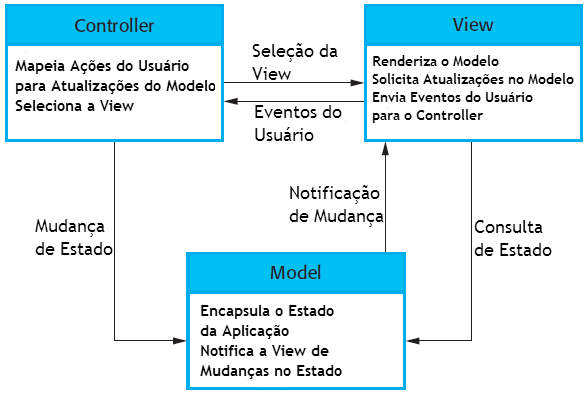
\includegraphics[scale=0.65]{imagens/mvc.png}
	\caption{A organização do MVC \citep{Sommerville10}.}
	\label{fig:mvc}
\end{figure} 

A Figura \ref{fig:mvc} mostra a relação entre essas camadas. As próximas subseções tem o objetivo de apresentar e explicar cada camada presente nesta arquitetura.

\subsection{Composição da Arquitetura}

Nesta subseção serão descritos os componentes presentes na arquitetura proposta, mostrando a função de cada um dentro da arquitetura, seus pontos de extensibilidade, bem como sua interação com elementos externos. Assim, facilitando o desenvolvimento da aplicação.

\subsubsection{Camada View}
A camada View contém as telas que mantêm a interação com o usuário. Esta camada é a responsável por enviar os eventos do usuário para a camada Controller, onde os eventos serão tratados e o fluxo seguinte da aplicação será selecionado.

\subsubsection{Camada Controller}

A camada Controller tem a responsabilidade de coordenar o fluxo da aplicação e fazer a integração entre as demais camadas. Responsável, também, por receber o processamento de um determinado componente e, com base no fluxo da aplicação, chamar o componente subsequente para dar continuidade ao processamento.

\subsubsection{Camada Model}
A camada Model é a camada de persistência de dados que contém as regras de acesso à base de dados e demais fontes de armazenamento de informações do sistema.





\section{Tecnologias}

Para o desenvolvimento do sistema foram utilizadas diversas tecnologias: linguagens de programação, servidores de aplicação e banco de dados, entre outras. A seguir apresentaremos estas tecnlogias.

\subsection{HTML, CSS e JavaScript}

HTML\footnote{https://www.w3.org/html} é uma linguagem de marcação utilizada para criação de páginas Web, criada por Tim Berners-Lee na década de 1990 \citep{Raggett:1998:RH:275611}. Sua sigla vem do inglês, abreviação para \textit{HyperText Markup Language}, que significa Linguagem de Marcação de Hipertexto. O HTML é uma linguagem para publicação de conteúdo (texto, imagem, vídeo, áudio etc.) na Web \citep{w3cHTML}. Ela foi utilizado para construir as páginas do sistema, que possibilitam a interação do usuário com o sistema. No \textit{framework} Laravel\footnote{https://laravel.com}, as páginas HTML são escritas utilizando um mecanismo de templates chamado Blade. A vantagem deste mecanismo é o esquema de herança de templates e seções que ele fornece, evitando assim reescrever o mesmo código em diversas páginas.

O CSS, \textit{Cascade Style Sheet}, é uma linguagem de folhas de estilo, responsável pelo layout das páginas web escritas em linguagens de marcação como o HTML. O CSS formata a informação entregue pelo HTML. Essa informação pode ser: imagem, texto, vídeo, áudio ou qualquer outro elemento criado. Ele permite formatar algumas características básicas: cores, \textit{background}, fontes, margens, \textit{paddings}, posição e assim controlamos de uma maneira muito
artesanal e simples a estrutura do site \citep{w3cCSS}.

Já o JavaScript é uma linguagem de programação utilizada para controlar o comportamento das páginas Web. A grande maioria dos websites modernos utilizam JavaScript, e todos os navegadores web modernos - em computadores, consoles de vídeo game, e smartphones - incluem interpretadores JavaScript \citep{flanagan2011javascript}. Ele foi desenvolvido pela Netscape em 1995, originalmente, chamado de LiveScript e fornecia uma linguagem de script simples para o navegador Netscape Navigator 2 \citep{ccmJS}. Ela permite que scripts sejam executados do lado do cliente em navegadores Web. Assim, a linguagem Javascript é altamente dependente do navegador que chama a página web onde o script está incorporado, mas, por outro lado, não requer nenhum compilador.

\subsection{PHP/Laravel e MySQL}

PHP\footnote{http://www.php.net} é uma linguagem interpretada, utilizada para o desenvolvimento de aplicações que rodam em servidores Web, capaz de gerar conteúdo dinâmico na Web. O código PHP é interpretado no lado do servidor, que gera uma página web, devolve para o lado cliente e então é exibida no navegador para o usuário. PHP originalmente era um acrônimo para \textit{Personal Home Page}, quando foi criada em 1994 por Rasmus Lerdorf para rastrear os visitantes de sua página. Com o crescimento de suas capacidades e utilidade, já que passou a ser utilizado em mais situações profissionais, veio a significar \textit{PHP: Hypertext Preprocessor} \citep{ullman2009php}.

O MySQL\footnote{https://www.mysql.com}, é um Sistema de Gerenciamento de Banco de Dados (SGBD), que utiliza a linguagem SQL (\textit{Structured Query Language}) como interface. Um banco de dados é uma coleção de dados inter-relacionados, sejam texto, números, ou arquivos binários, que são armazenados e mantidos organizados por um SGBD \citep{ullman2009php}. Ao incorporar um banco de dados em uma aplicação Web, alguns dos dados gerados pelo PHP podem ser recuperados do MySQL, como ilustra a Figura \ref{fig:php-mysql}.

\begin{figure}
	\centering
	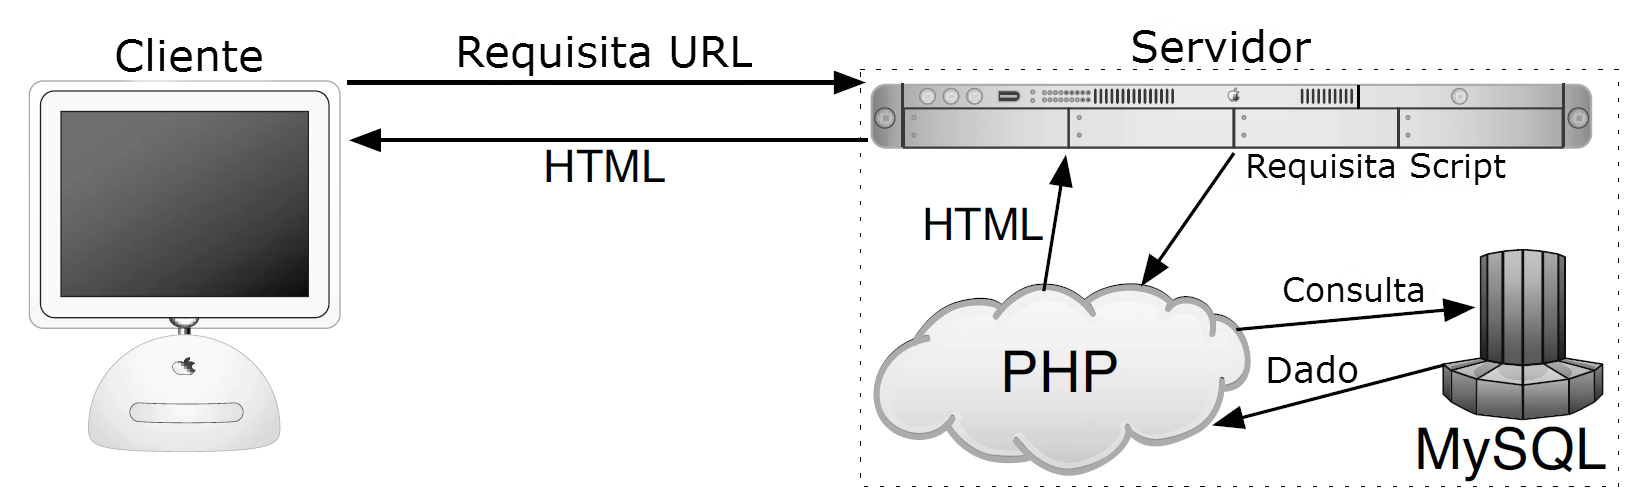
\includegraphics[scale=0.2]{imagens/php-mysql.png}
	\caption{Funcionamento de aplicações Web dinâmicas, utilizando PHP e Mysql \citep{ullman2009php}.}
	\label{fig:php-mysql}
\end{figure}

O sistema foi desenvolvido utilizando o Laravel\footnote{https://laravel.com}, um framework de desenvolvimento web para a linguagem PHP, que utiliza o padrão MVC. Ele possui um sistema modular com gerenciador de dependências, vários modos de acesso a bancos de dados e diversos utilitários que ajudam no desenvolvimento do sistema. Assim, o benefício de utilizar um framework em geral é que, além de trazer vários componentes individuais, também já fornece uma integração entres esses componentes. Adicionalmente, fornecem convenções que reduz a quantidade de código que um desenvolvedor novo em um projeto precisa entender \citep{stauffer2016laravel}.

O MySQL possui fácil integração com o PHP e, através do Laravel, a configuração se torna bastante trivial. O projeto possui um arquivo de configuração chamado "database.php", onde são informados os dados de conexão do banco de dados. Em relação ao gerenciamento da estrutura do banco de dados, o Laravel utiliza Migrations para manter a estrutura das tabelas do banco de dados. Migrations possibilitam o controle de versão do banco de dados, e assim permite a uma equipe facilmente modificar e compartilhar o esquema do banco, além de permitir facilmente criar todo o banco de dados através de uma comando. A Figura \ref{fig:banco-dados} ilustra os itens presentes no dataset.

\begin{figure}
	\centering
	\advance\leftskip-2cm
	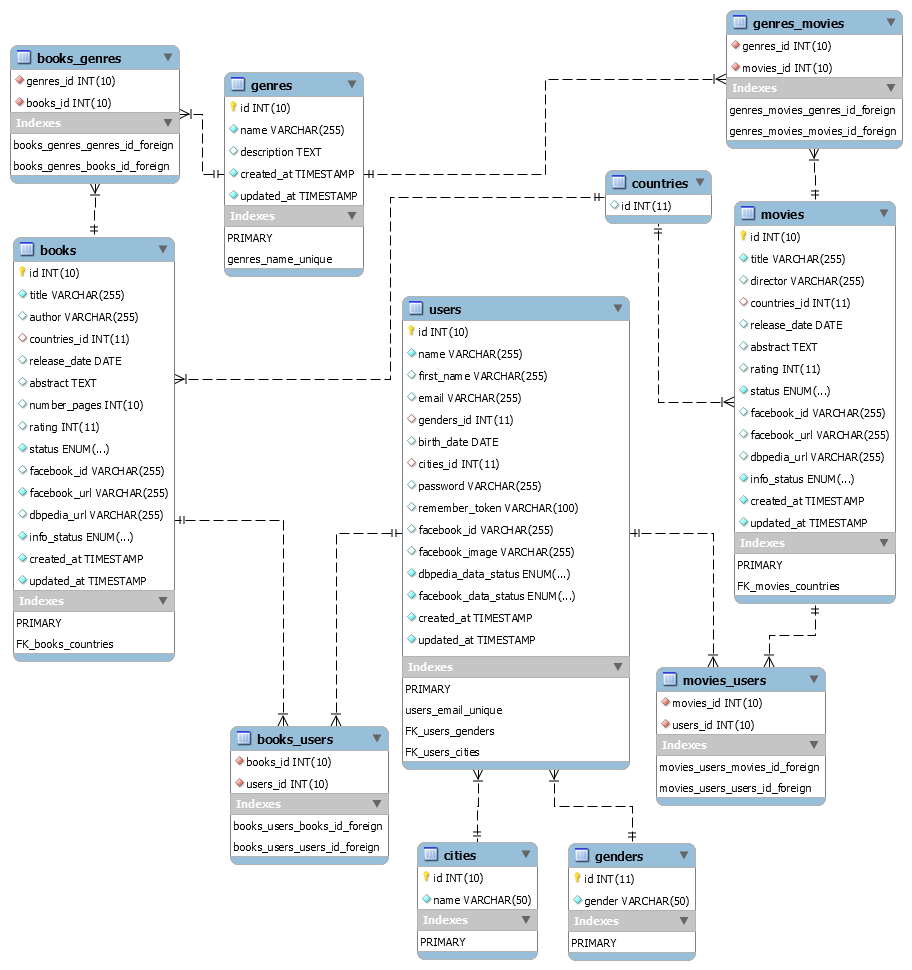
\includegraphics[scale=0.61]{imagens/banco.png}
	\caption{Diagrama Entidade-Relacionamento do Sistema. Figura elaborada pelo autor (2015).}
	\label{fig:banco-dados}
\end{figure}





\subsection{SPARQL}

SPARQL, acrônimo recursivo para \textit{SPARQL Protocol and
RDF Query Language}, é uma linguagem de consulta semiestruturada semântica para banco de dados, capaz de recuperar e manipular dados armazenados em RDF, \textit{Resource Description Framework}. RDF é um modelo de dados em que você expressa fatos com declarações de três partes, conhecidas com triplas. Cada tripla é como uma pequena frase que afirma um fato. Essas triplas são compostas de \textit{sujeito}, que é o identificador da coisa sendo descrita, \textit{predicado}, representa o nome da propriedade, e \textit{objeto}, que é o valor da propriedade \citep{ducharme2011sparql}.

Para a realização do enriquecimento de informações sobre os filmes e livros do usuário, foi utilizada a \textit{SPARQL RDF Library for PHP}\footnote{http://graphite.ecs.soton.ac.uk/sparqllib/}, que é uma biblioteca em PHP para realizar consultas SPARQL. O Código Fonte \ref{cod:sparql-movie} mostra a consulta utilizando SPARQL para obter informações sobre um filme. A cláusula \textit{SELECT}, na linha 7, é utilizada para extrair os valores da base RDF. O \textit{SELECT} foi utilizado em combinação com \textit{DISTINCT}, que elimina soluções duplicadas. Da linha 8 até a linha 15 estão as variáveis para cada um dos predicados que desejamos obter. Os resultados desta consulta serão apresentados em uma tabela.

Inicialmente definimos alguns prefixos, o que nos permite evitar ter que escrever as URIs, \textit{Uniform Resource Identifier} completas nas triplas. A consulta utiliza algumas triplas dentro da cláusula \textit{WHERE} para indicar o subconjunto de dados que queremos. Cada tripla termina com um ponto e tem um sujeito \textit{?film\_title}. A primeira tripla, na linha 18, consulta por todas as instâncias da classe \textit{Film}. E das linhas 19 a 22 solicitamos os predicados \textit{rdfs:comment}, \textit{dct:subject}, \textit{rdfs:label} que representam a sinopse, gênero e nome do filme, respectivamente. A palavra-chave \textit{OPTIONAL} permite trazer resultados opcionais, sem essa palavra-chave, um processador SPARQL irá retornar apenas dados que correspondam a cada tripla da cláusula \textit{WHERE}. No nosso caso, solicitamos como opcionais \textit{dbo:director}, \textit{dbpprop:country}, \textit{dbpprop:released}, \textit{dbo:runtime}, que representam o diretor, país, data de lançamento e duração do filme, respectivamente.

Foi utilizada, também, a cláusula \textit{FILTER} para filtrar os resultados apenas para o idioma inglês, linhas 28 a 30, e na linha 31 um filtro onde informamos o nome do filme que desejamos consultar.

\begin{lstlisting}[caption=Consulta SPARQL para um Filme., language=SPARQL, frame=single, label={cod:sparql-movie}, float, numbers=left]
PREFIX rdf: <http://www.w3.org/1999/02/22-rdf-syntax-ns#>
PREFIX rdfs: <http://www.w3.org/2000/01/rdf-schema#>
PREFIX dbpedia: <http://dbpedia.org/resource/>
PREFIX dbo: <http://dbpedia.org/ontology/>
PREFIX dbpprop: <http://dbpedia.org/property/>

SELECT DISTINCT
str(?name) as ?film_title
str(?film_director) as ?film_director
str(?film_country) as ?film_country
str(?film_released) as ?film_released
str(?film_abstract) as ?film_abstract
?film_runtime
(group_concat(distinct ?film_genre;separator=",") 
as ?film_genre)

WHERE {
?film_title rdf:type <http://dbpedia.org/ontology/Film> .
?film_title rdfs:comment ?film_abstract .
?film_title dct:subject/rdfs:label ?film_genre .
?film_title rdfs:label ?name
OPTIONAL {
?film_title dbo:director/rdfs:label ?film_director .
?film_title dbpprop:country ?film_country .
?film_title dbpprop:released ?film_released .
?film_title dbo:runtime ?film_runtime .
}
FILTER(LANGMATCHES(LANG(?name), "en")) .
FILTER(LANGMATCHES(LANG(?film_director), "en")) .
FILTER(LANGMATCHES(LANG(?film_abstract), "en")) .
FILTER contains(str(?name), "Titanic")
}
\end{lstlisting}

\subsection{Facebook API}
A API\footnote{https://developers.facebook.com} do Facebook é uma plataforma para construir aplicações que estarão disponíveis para usuários da rede social Facebook. A API permite que aplicações façam uso das conexões sociais e informações do perfil do usuário. A API foi utilizada para a realização de autenticação na aplicação e obtenção dos filmes e livros do usuário.







\begin{figure}
	\centering
	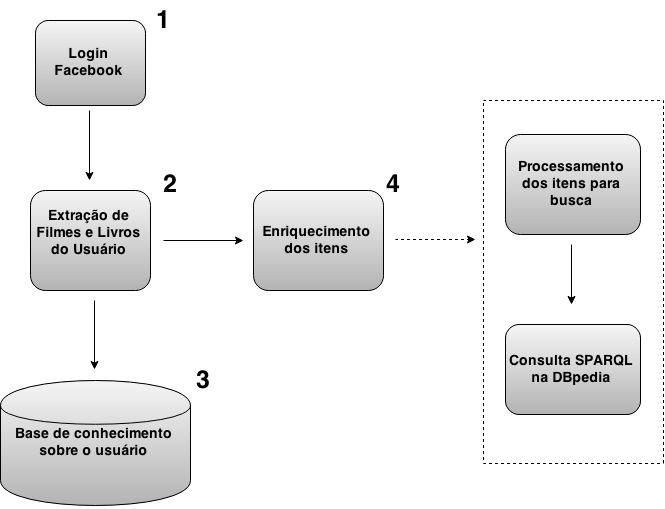
\includegraphics[scale=0.6]{imagens/arquitetura.png}
	\caption{Fluxo do Funcionamento do Sistema. Figura elaborada pelo autor (2015).}
	\label{fig:funcionamento}
\end{figure}



\section{Telas e Funcionamento}

O sistema foi desenvolvido para funcionar como um \textit{website}, e possui  um visual em que apresenta galerias de filmes e livros do usuário. A princípio utiliza-se de dados sobre o interesse do usuário em filmes e livros obtidos no Facebook. A Figura \ref{fig:funcionamento} apresenta um fluxograma com uma visão geral do funcionamento do sistema.

Inicialmente (Passo 1 da Figura \ref{fig:funcionamento}) o usuário deve realizar login no sistema utilizando sua conta do Facebook, como pode ser visto na Figura \ref{fig:sis-login}. Para realizar o login no sistema, o usuário precisa, necessariamente ter uma conta no Facebook. Neste momento serão obtidos dados básicos do usuário, como nome, email e data de nascimento. Uma vez logado, o usuário consegue ter acesso a todas as informações existentes no aplicativo e só precisará passar novamente pelo processo de \textit{login} caso opte por se desconectar do sistema, processo popularmente conhecido como \textit{logout}. Isso acontece porque o sistema guarda o estado do usuário do sistema, o que significa dizer que se o mesmo está logado não precisa passar pelo processo de autenticação novamente.

\begin{figure}[H]
	\centering
	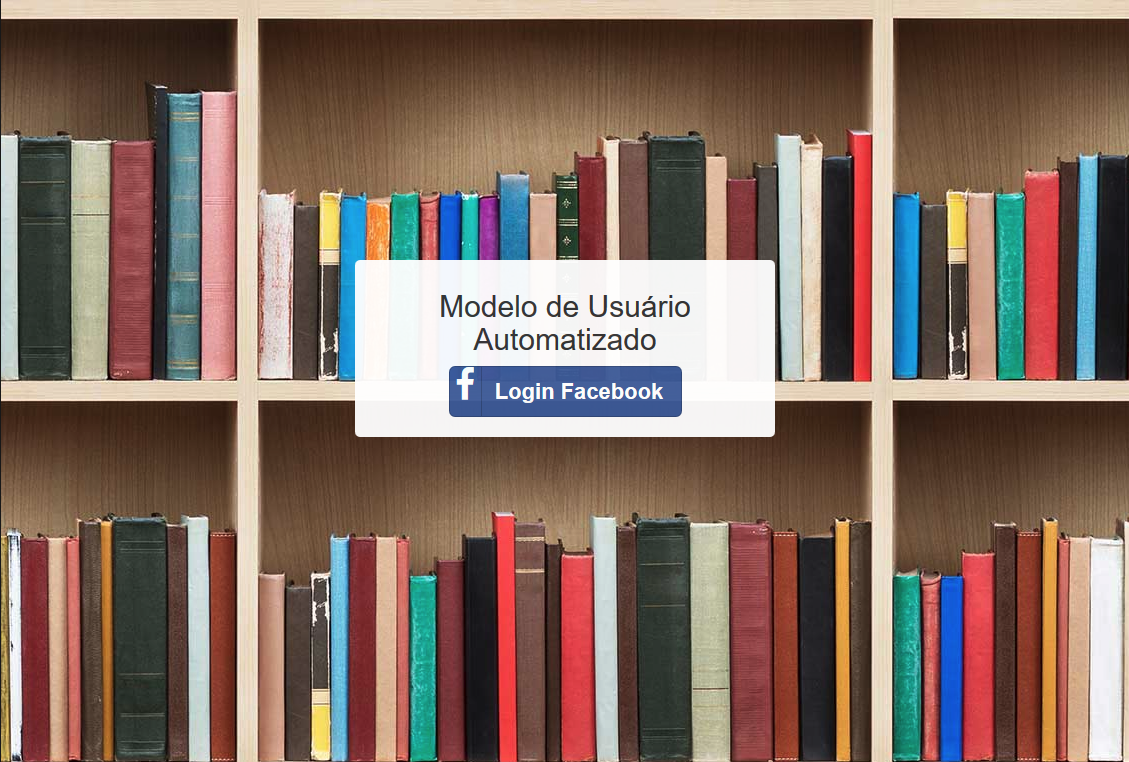
\includegraphics[scale=0.5]{imagens/sistema/login.png}
	\caption{Tela de login de usuário. Figura elaborada pelo autor (2015).}
	\label{fig:sis-login}
\end{figure}

Após ter acesso ao sistema, o usuário verá a opção de coletar seus dados de livros e filmes do Facebook, como visto na Figura \ref{fig:sis-coletar}. Quando o usuário acessar a opção para coletar seus dados do Facebook, o sistema irá coletar todos os filmes e livros que foram marcados pelo usuário como "assistidos"~ ou "lidos". Também, neste momento é realizada uma consulta ao Facebook, nas páginas de cada filme, para obter a data de lançamento de cada filme e livro. Esses dados são então armazenados em um banco de dados, relacionando-os ao usuário (Parte 3 da Figura \ref{fig:funcionamento}), montando uma base de conhecimento inicial sobre o usuário.

\begin{figure}
	\centering
	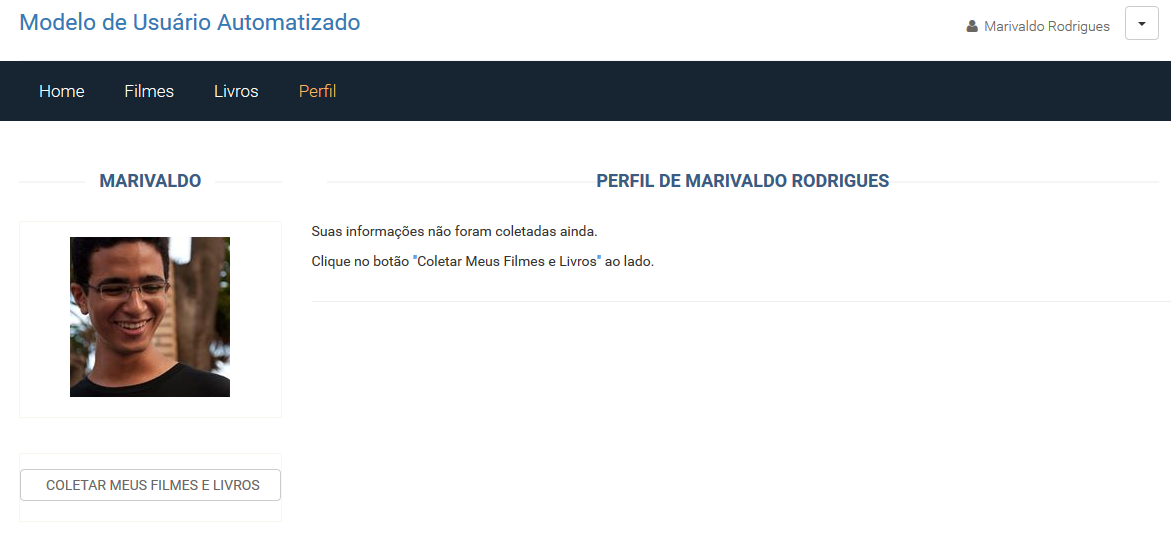
\includegraphics[scale=0.5]{imagens/sistema/usuario-coletar.png}
	\caption{Tela do perfil do usuário com opção para coleta dos dados. Figura elaborada pelo autor (2015).}
	\label{fig:sis-coletar}
\end{figure}

Até este momento temos apenas uma relação com os nomes dos filmes e livros do usuário. Precisamos agora obter mais informações sobre esses itens, para poder entender o que eles representam, e o seu significado para o usuário. Assim, é feito um enriquecimento de informações sobe os itens do usuário (Parte 4 da Figura \ref{fig:funcionamento}). Para isso foi utilizado a base da DBpedia\footnote{http://wiki.dbpedia.org} como fonte. Então, o sistema deve checar cada item que não possua detalhes e consultar a base da DBPedia para complementar essas informações.

O sistema possui uma tela, ilustrada na  Figura \ref{fig:sis-livro-detalhes}, onde o usuário pode acessar a página de um livro ou filme e visualizar os detalhes das informações deste item. Também é possível visualizar uma lista com todos os filmes e livros que foram coletados pelo sistema, como pode ser visto na Figura \ref{fig:sis-filmes}.


\begin{figure}[H]
	\centering
	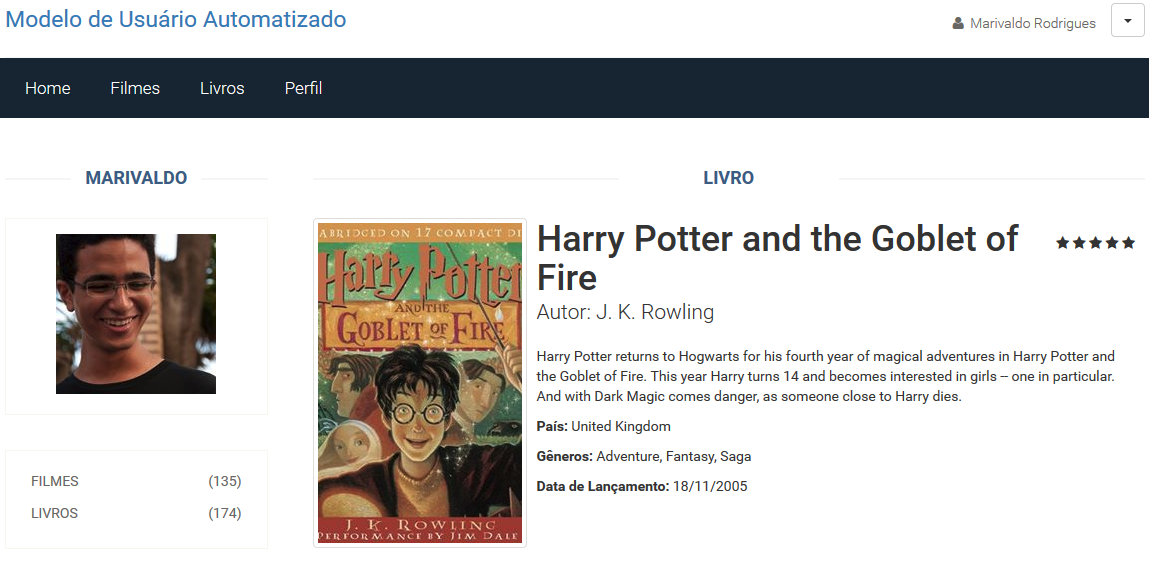
\includegraphics[scale=0.5]{imagens/sistema/usuario-livro-detalhes.png}
	\caption{Tela de visualização dos detalhes de um livro. Figura elaborada pelo autor (2015).}
	\label{fig:sis-livro-detalhes}
\end{figure}


\begin{figure}
	\centering
	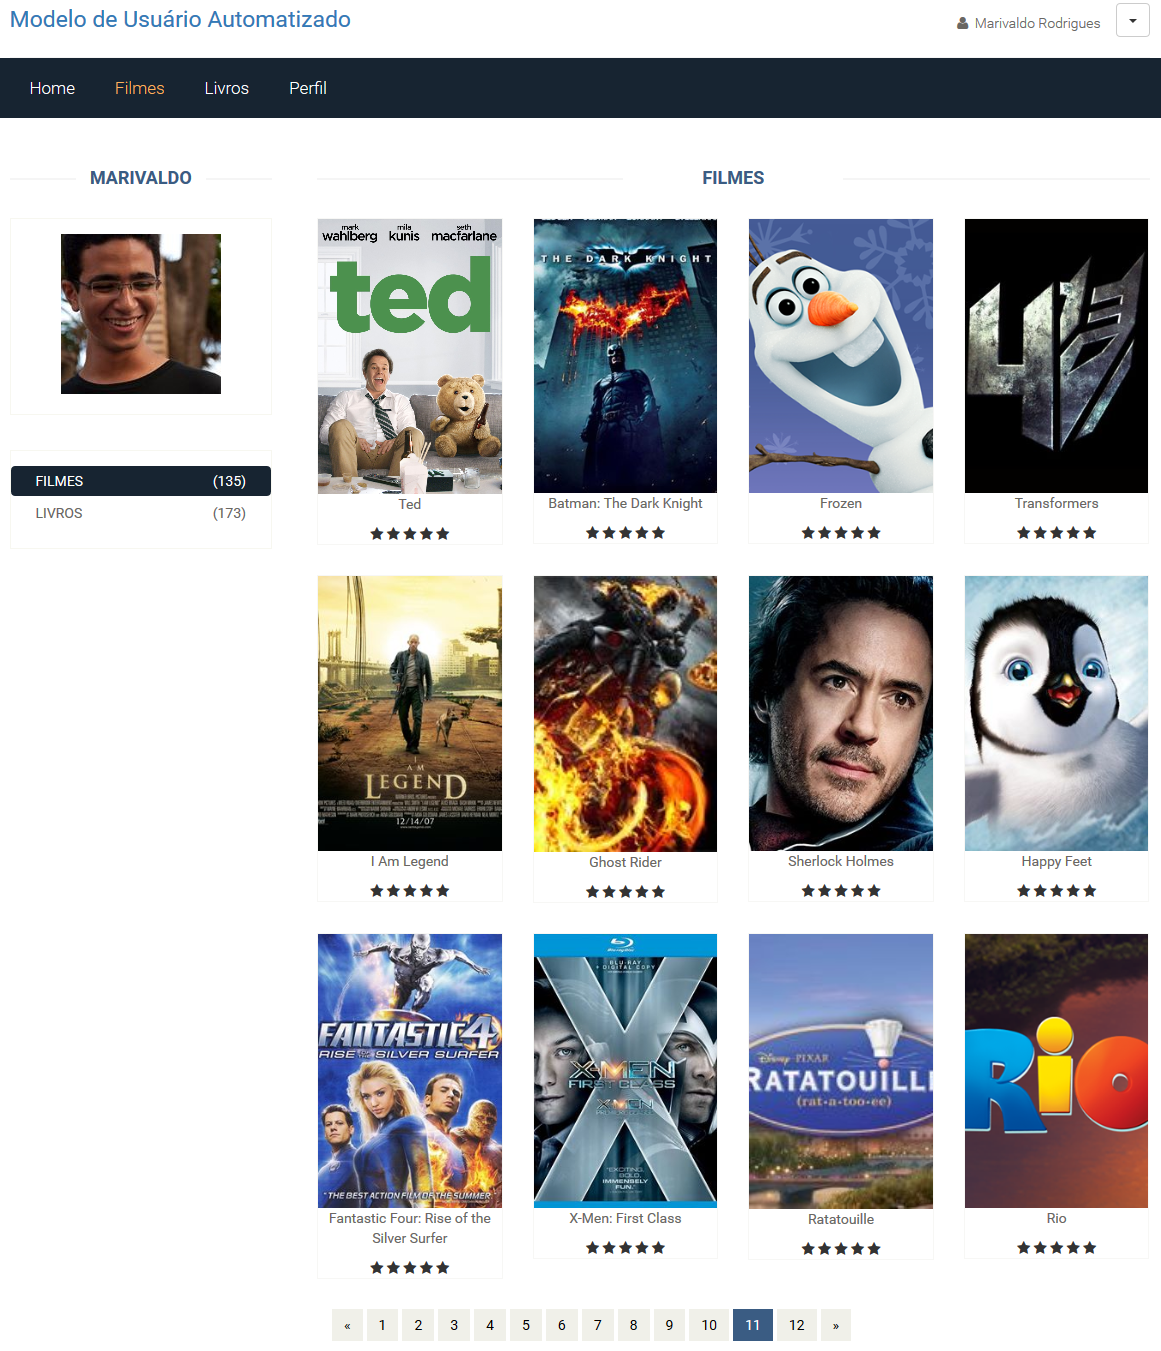
\includegraphics[scale=0.4]{imagens/sistema/usuario-filmes.png}
	\caption{Tela de visualização dos filmes do usuário. Figura elaborada pelo autor (2015).}
	\label{fig:sis-filmes}
\end{figure}

As consultas são realizadas através dos títulos de cada item. Antes de realizar a consulta é realizado um processo de "limpeza"~ nos títulos dos itens para remover alguns padrões, com o objetivo de facilitar a descoberta do item. Por exemplo "O Poderoso Chefão (1972)", nesse caso é removido o ano do filme ficando "O Poderoso Chefão". Os detalhes buscados sobre os itens são: gêneros, sinopse, diretor, atores, data de lançamento, duração. Sendo considerado a informação mais importante o gênero do item, que será utilizado como "ponte"~ entre os domínios.

Após todos os filmes e livros estarem com todas as informações preenchidas, o usuário poderá visualizar uma página com os gêneros de filmes e livros que ele mais costuma assistir e ler, respectivamente, conforme pode ser visto na Figura \ref{fig:sis-perfil}.

\begin{figure}[H]
	\centering
	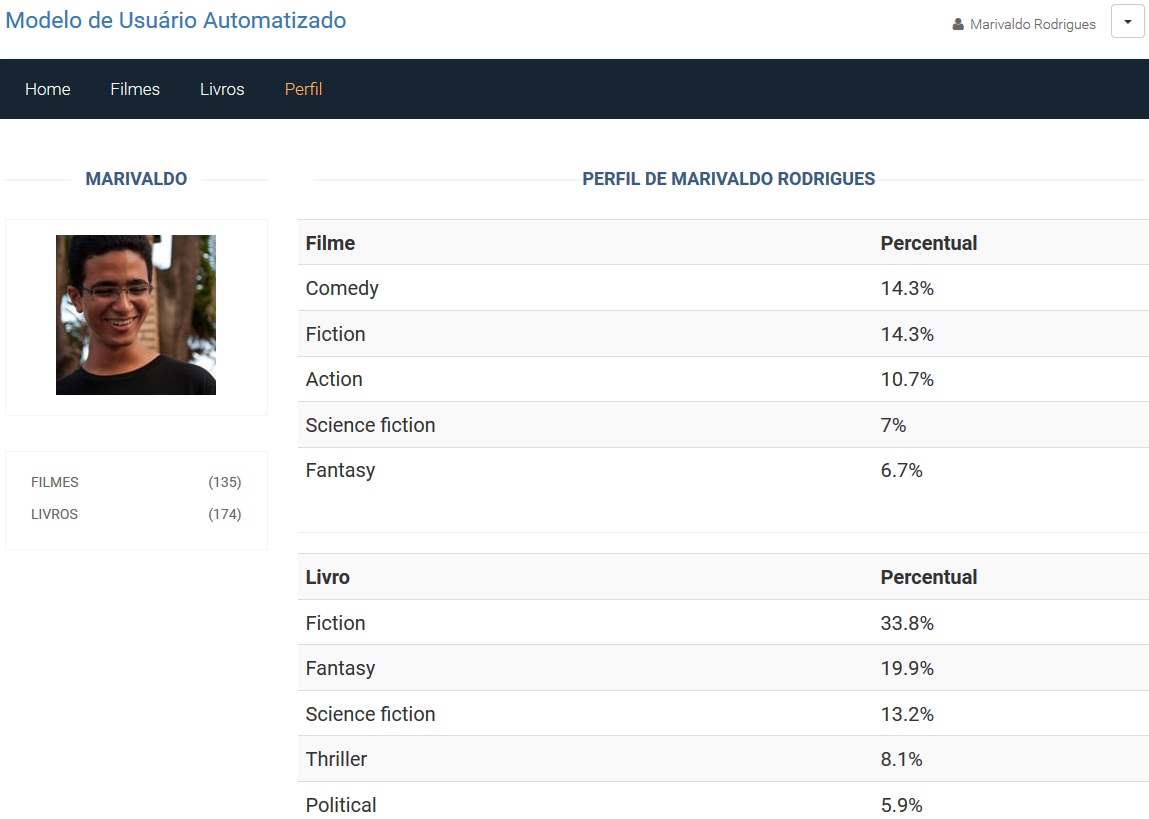
\includegraphics[scale=0.45]{imagens/sistema/usuario-perfil.png}
	\caption{Tela do perfil com estatísticas de gêneros mais assistidos e lidos pelo usuário. Figura elaborada pelo autor (2015).}
	\label{fig:sis-perfil}
\end{figure}







\section{Sumário}

Neste capítulo, apresentamos uma visão geral sobre os aspectos do desenvolvimento do sistema. Inicialmente discutimos a arquitetura do sistema, onde vimos os aspectos da estrutura do sistema. Em seguida, vimos as ferramentas e tecnologias utilizadas e depois o fluxo de funcionamento foi explicado. No capítulo \ref{cap:avaliacao} faremos uma avaliação do trabalho realizado. Serão discutidas metodologia, métricas de avaliação e os resultados obtidos.